\chapter{Installationsanleitung}
Dies ist die Installationsanleitung für den Smartmanager. Der Smartmanager unterstützt eine Installation unter Linux sowie auch unter Windows. Ein Deployment in einer PaaS wird momentan noch nicht unterstützt. 
\section{Benötigte Software}
Für die Installation der Applikation werden folgende Softwares benötigt:
\begin{itemize}
\item Java SE Runtime Environment Version 8
\item Tomcat Version 8
\item Maven
\item git
\end{itemize}
\section{Zertifikat Variante 1: PKI}
\subsubsection{Keystore erstellen}
Als ersten Schritt erstellt man mit dem Keytool einen Keystore. Diese benötigt einen Alias und einen Pfad, indem er abgelegt wird. Dieser Pfad wird später für die Applikationskonfiguration benötigt.
  
Nun wird man nach einem Passwort gefragt. Dieses wird auch für die spätere Applikationskonfiguration benötigt.
\begin{figure}[H]
\centering
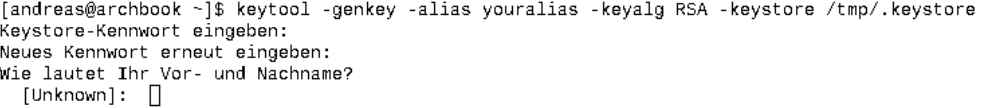
\includegraphics[scale=0.65]{../05_Schlussbericht/images/keystore1.png}
\end{figure}
Danach gibt man alle wichtig Informationen zum Zertifikat an. Diese Informationen müssen alle stimmen, da diese an die ''Certificate Authority'' weitergegeben werden. Dies kann am Schluss mit ''Ja'' bestätigt werden.
\begin{figure}[H]
\centering
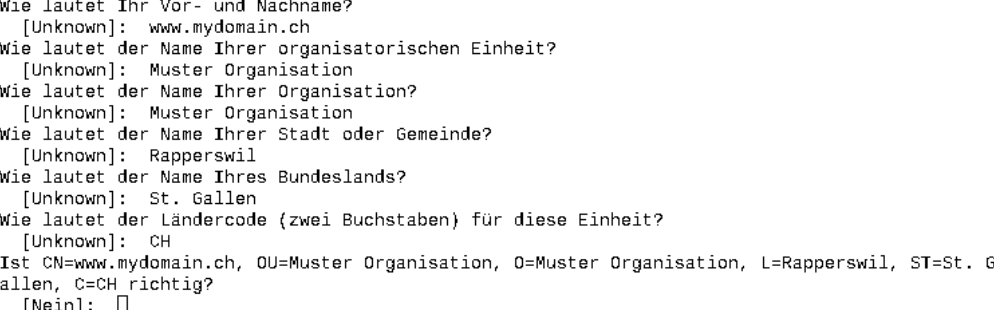
\includegraphics[scale=0.65]{../05_Schlussbericht/images/keystore2.png}
\end{figure}

Zum Schluss wird nun noch ein Password verlangt, welches für dieses Zertifikat gilt. Dies muss das gleiche Password wie für den Store sein, da Tomcat sonst nicht auf das Zertifikat zugreifen kann.

\subsubsection{CSR erstellen}
Als nächsten Schritt wird der Certificate Signing Request erstellt. Dazu gibt man folgenden Befehl ein:
\begin{figure}[H]
\centering
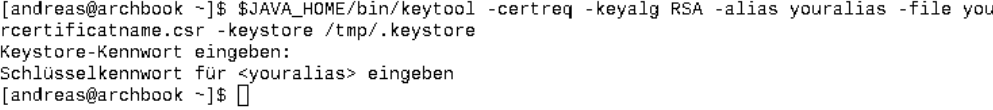
\includegraphics[scale=0.65]{../05_Schlussbericht/images/keystore3.png}
\end{figure}


Dieses Zertifikat kann man nun bei einer ''Certificate Authority'' bestätigen lassen und erhält danach die benötigten Zertifikate.
\subsubsection{Zertifikate importieren}
Die erhaltenen Zertifikate werden nun importiert. Zuerst wird das Root-Zertifikat importiert.
\begin{figure}[H]
\centering
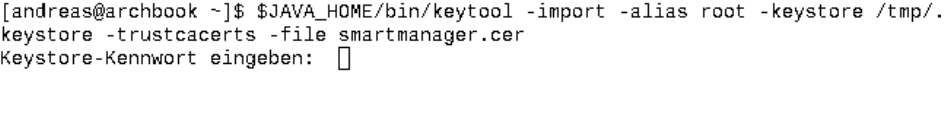
\includegraphics[scale=0.65]{../05_Schlussbericht/images/keystore4.png}
\end{figure}

Danach import man das erhaltene Zertifikat und gibt die Passwörter ein. Durch das ist der Keystore vorbereitet.
\begin{figure}[H]
\centering
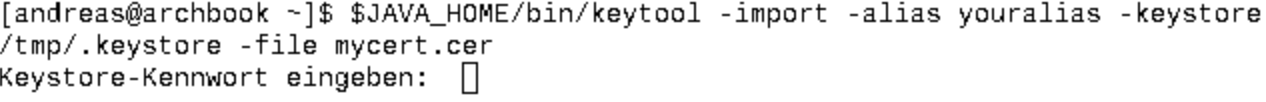
\includegraphics[scale=0.4]{../05_Schlussbericht/images/keystore5.png}
\end{figure}
\section{Zertifikat Variante 2: Self-Signed}
Anstelle einer PKI kann man auch einfach ein Self-Signed Zertifikat erstellen. Durch diesen Befehl ist dies Möglich:
\begin{figure}[H]
\centering
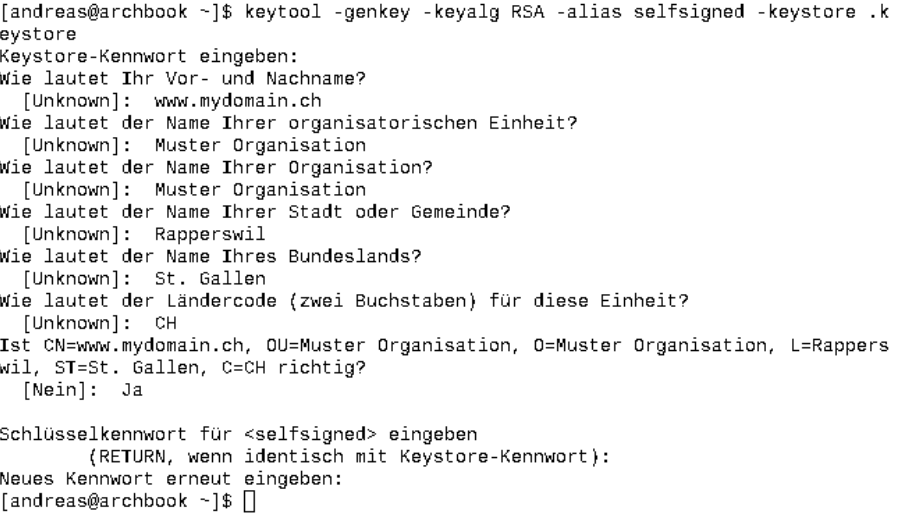
\includegraphics[scale=0.65]{../05_Schlussbericht/images/keystore6.png}
\end{figure}

Dies reicht aus, damit Tomcat auf das Zertifikat zugreifen kann.



\section{Smartmanager}
\subsubsection{Smartmanager herunterladen}
Das Projekt befindet sich auf folgendem URL: \href{https://github.com/BA-Smartmanager/smartmanager}{https://github.com/BA-Smartmanager/smartmanager}

Durch ''git clone https://github.com/BA-Smartmanager/smartmanager'' kann nun das Repo heruntergeladen werden.

\subsubsection{Smartmanager konfigurieren}
Im erhaltenen Ordner smartmanager befindet sich nun der gesamte Source-Code. Um Einstellungen vorzunehmen, öffnet man die Datei ''smartmanager/WebContent/WEB-INF/smartmanager-configuration.xml''

In dieser Datei kann die LwM2M-Server Adresse und die MongoDB-URL anpassen. Weitere Einstellungen sind nicht nötig.
\begin{lstlisting}[language=xml]
<property name="address" value="127.0.0.1" />
<property name="port" value="5683"></property>
		
<mongo:db-factory id="mongoDbFactory" client-uri="mongodb://localhost/smartmanager" />
\end{lstlisting}

\subsubsection{Builden}
Um die Software zu builden, gibt im Ordner ''smartmanager'' ''mvn clean install'' ein. Diese generiert ein Ordner target und darin befindet sich eine .war-Datei. Diese wird später in den Tomcat-Ordner kopiert. Am besten bennent man diese .war-Datei in ''smartmanager.war'' um, da dieser Name die URL direkt beeinflusst.

\subsection{Tomcat}
\subsubsection{Konfigurieren}
Im Tomcat Installationsverzeichnis befindet sich im Ordner ''conf'' die Datei server.xml. In dieser sucht man nach den Connector Tags und fügt folgende hinzu.
\begin{lstlisting}[language=xml]
<Connector port="8080" protocol="HTTP/1.1" connectionTimeout="20000" redirectPort="8443" />

<Connector port="8443" protocol="org.apache.coyote.http11.Http11NioProtocol"
	maxThreads="150" SSLEnabled="true" scheme="https" secure="true"
	clientAuth="false" sslProtocol="TLS" keystoreFile="</yout/keystore/path/.keystore>"
	keystorePass="<Your Password>">
</Connector>
\end{lstlisting}

Dabei ist wichtig, dass der Pfad zum Keystore, sowie das dazugehörige Passwort richtig angegeben werden.
Sollten noch weitere Connector Einträge wie folgender vorhanden sein (Nur die mit Port 8080):
\begin{lstlisting}[language=xml]
<Connector port="8080" protocol="HTTP/1.1" connectionTimeout="20000" redirectPort="8443" />
\end{lstlisting}
können diese gelöscht werden.
\subsubsection{War-Datei in Tomcat einfügen}
Die vorher erstellte .war-Datei wird nun kopiert und in den ''/webapps/''-Ordner im Tomcat Installationsverzeichnis eingefügt.
\subsubsection{Tomcat starten}
Zum Schluss wird nun Tomcat gestartet. Dies kann man durch die im Tomcat Installationsverzeichnis vorhandenen Skripts erledigen. Zu finden sind diese im ''bin''-Ordner
